\documentclass{../cscslides}

\slidetitle{Лекция 10: Предметно-ориентированное проектирование}{18.04.2022}

\begin{document}
    
    \frame{\titlepage}

    \section{Введение}

    \begin{frame}
        \frametitle{Domain-Driven Design}
        \textbf{Domain-Driven Design} --- модная нынче методология проектирования, использующая предметную область как основу архитектуры системы
        \begin{itemize}
            \item Архитектура приложения строится вокруг \textbf{Модели предметной области}
            \item Модель определяет \textbf{Единый язык}, на котором общаются и разработчики, и эксперты, описывая естественными фразами то, что происходит и в программе, и в реальности
            \item Модель --- это не только диаграммы, это ещё (и прежде всего) код, и устное общение
        \end{itemize}
        DDD даёт ответ на вопрос ``откуда брать эти все классы'' и позволяет целенаправленно уточнять и улучшать архитектуру системы. 
        Особенно полезно, когда предметная область не очень знакома.
    \end{frame}

    \begin{frame}
        \frametitle{Книжка}
        Эрик Эванс, ``Предметно-ориентированное проектирование. Структуризация сложных программных систем''. М., ``Вильямс'', 2010, 448 стр.
        \begin{center}
            
\includegraphics[width=0.25\textwidth]{dddCover.jpg}
        \end{center}
    \end{frame}

    \section{Пример}

    \begin{frame}
        \frametitle{Domain-Driven Design, анализ}
        \framesubtitle{Пример: печатные платы}
        \begin{center}
            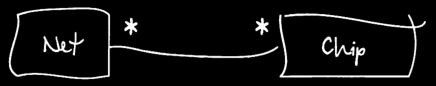
\includegraphics[width=0.6\textwidth]{netClassesBlack.png}

            \bigskip

            \bigskip
            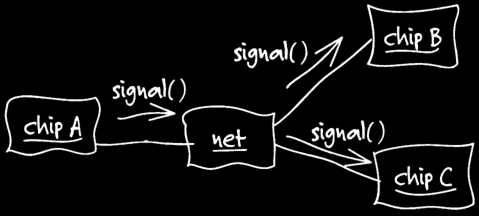
\includegraphics[width=0.6\textwidth]{netObjectsBlack.png}
        \end{center}
    \end{frame}

    \begin{frame}
        \frametitle{Печатные платы, топология}
        \begin{center}
            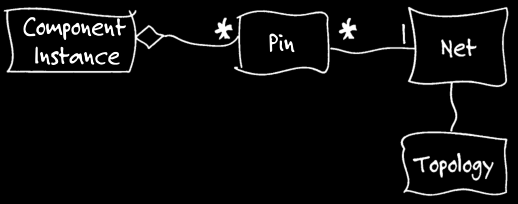
\includegraphics[width=0.7\textwidth]{topologyBlack.png}
        \end{center}
    \end{frame}

    \begin{frame}
        \frametitle{Печатные платы, сигналы}
        \begin{center}
            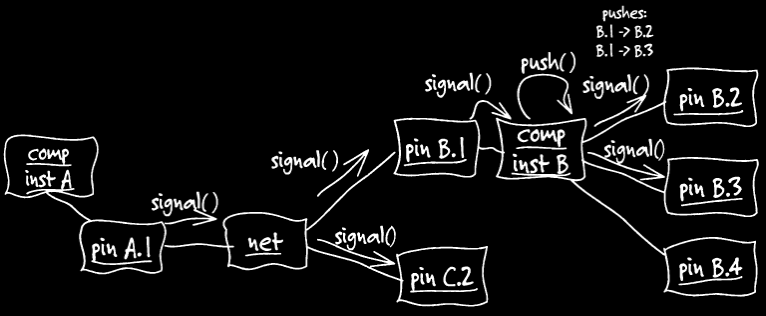
\includegraphics[width=0.9\textwidth]{signalsBlack.png}
        \end{center}
    \end{frame}

    \begin{frame}
        \frametitle{Печатные платы, прозванивание}
        \begin{center}
            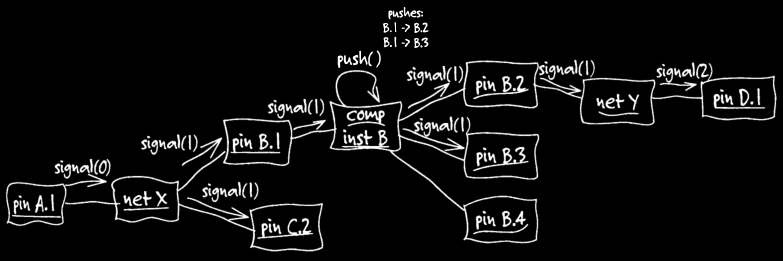
\includegraphics[width=\textwidth]{probeSimulationBlack.png}
        \end{center}
    \end{frame}

    \begin{frame}
        \frametitle{Печатные платы, типы}
        \begin{center}
            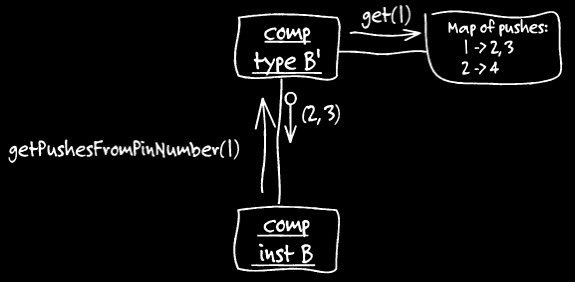
\includegraphics[width=0.7\textwidth]{typesBlack.png}
        \end{center}
    \end{frame}

    \begin{frame}
        \frametitle{Печатные платы, модель}
        \begin{center}
            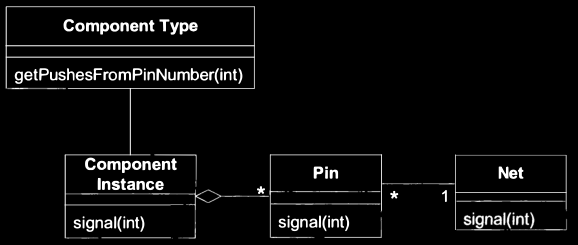
\includegraphics[width=0.8\textwidth]{finalModelBlack.png}
        \end{center}
    \end{frame}

    \begin{frame}
        \frametitle{Выводы: правила игры}
        \begin{itemize}
            \item Детали реализации не участвуют в модели
            \begin{itemize}
                \item ``База данных? Какая база данных?''
            \end{itemize}
            \item Должно быть можно общаться, пользуясь только именами классов и методов
            \item Не нужные для текущей задачи сущности предметной области не должны быть в модели
            \item Могут быть скрытые сущности, которые следует выделить явно
            \begin{itemize}
                \item при этом объяснив экспертам их роль в реальной жизни и послушав их мнение
                \item например, различные ограничения могут стать отдельными классами
            \end{itemize}
            \item Диаграммы объектов могут быть очень полезны
        \end{itemize}
    \end{frame}

    \section{Единый язык}

    \begin{frame}
        \frametitle{Единый язык}
        \begin{itemize}
            \item У программистов и специалистов предметной области свой профессиональный жаргон
            \item Свои жаргоны появляются даже среди групп разработчиков в одном проекте
            \item Необходимость перевода размывает смысл понятий
            \item ``Еретики'' используют понятия в разных смыслах
            \item Единый язык --- понятия из модели (классы, методы), паттерны, элементы ``высокоуровневой'' структуры системы (которая не отражается в коде)
            \item Изменения в языке --- рефакторинг кода
            \item Языков в проекте может быть много
        \end{itemize}
    \end{frame}

    \begin{frame}
        \frametitle{Без единого языка}
        \begin{center}
            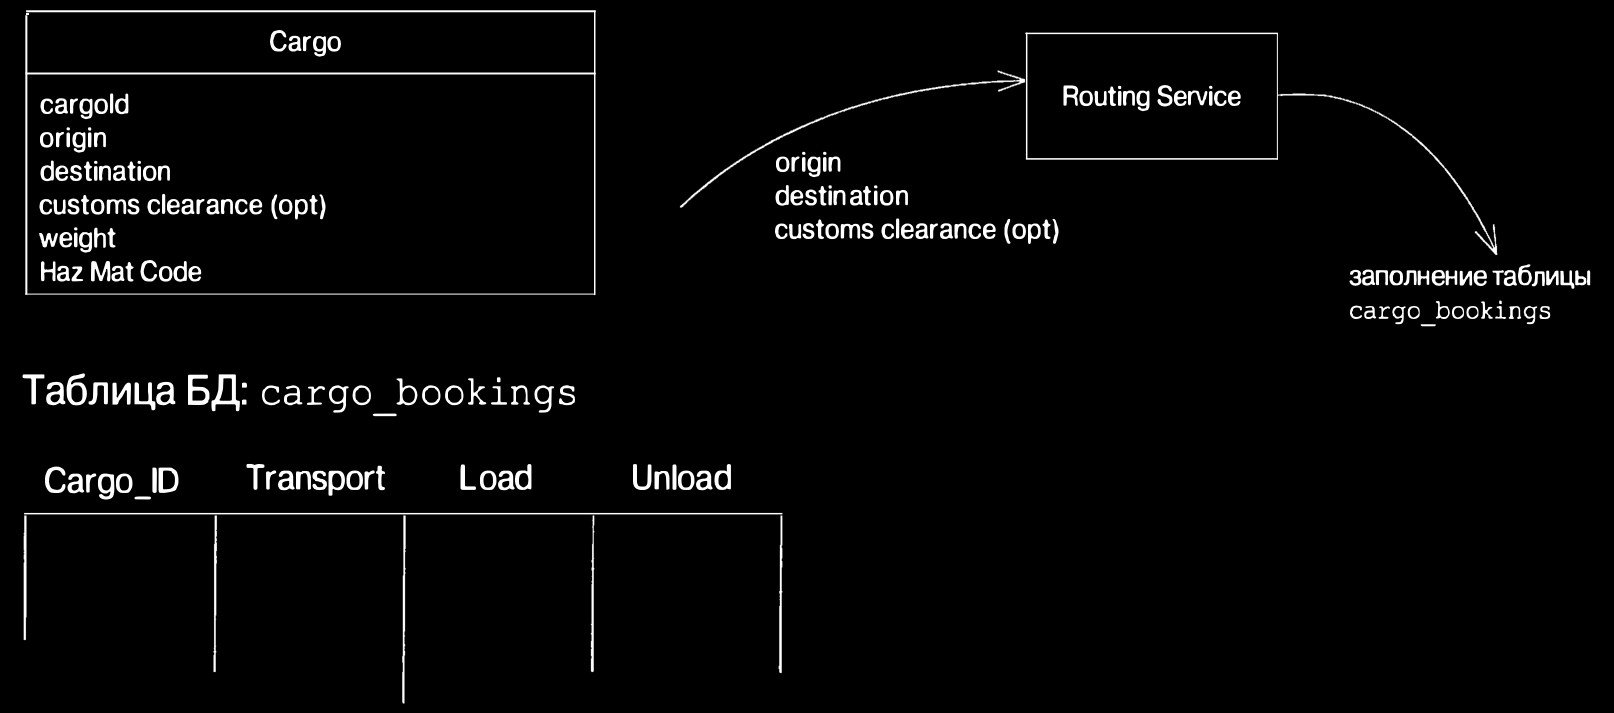
\includegraphics[width=0.9\textwidth]{lowAbstractionLanguageBlack.png}
        \end{center}
    \end{frame}

    \begin{frame}
        \frametitle{С единым языком}
        \begin{center}
            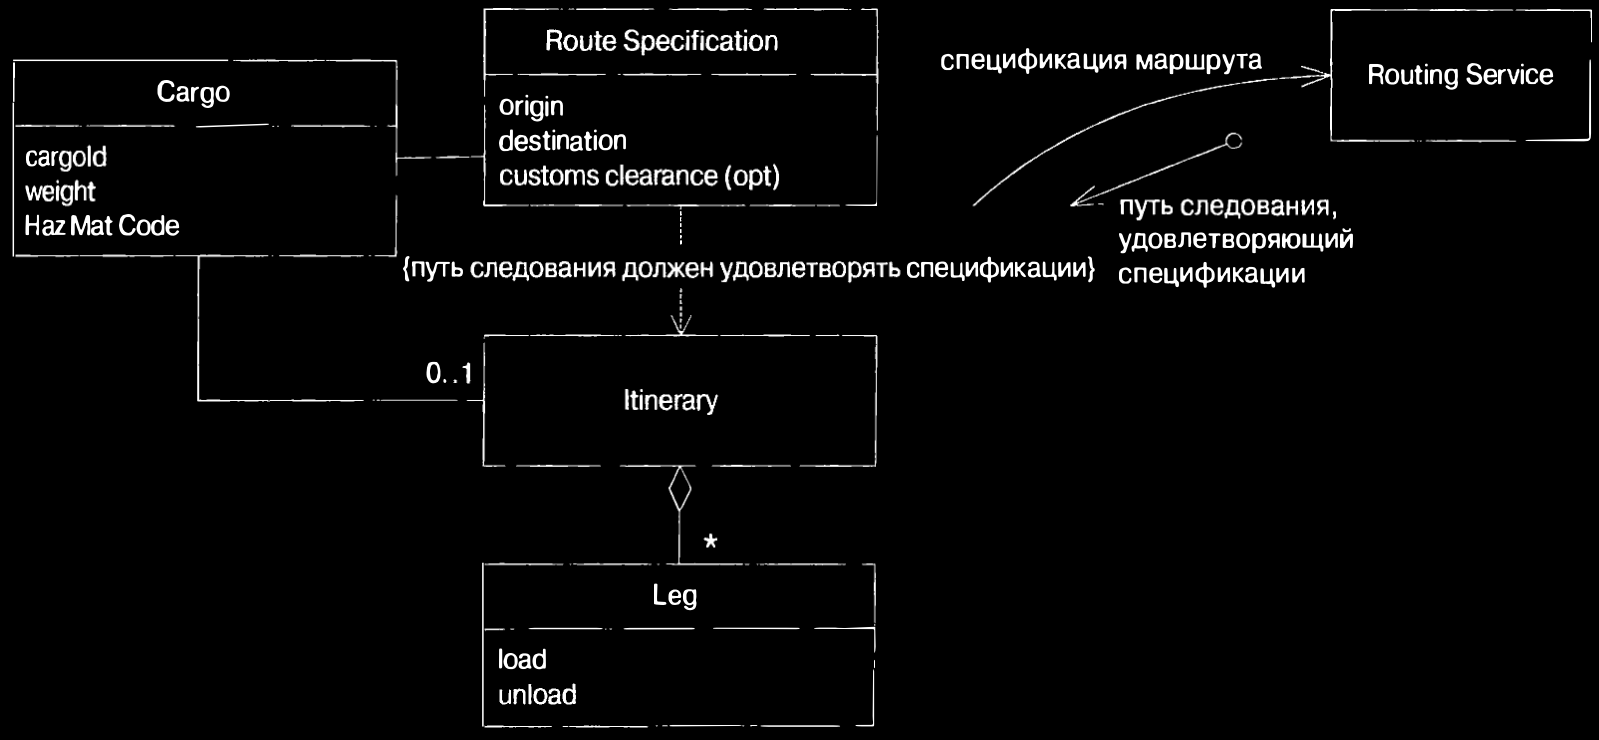
\includegraphics[width=0.9\textwidth]{highAbstractionLanguageBlack.png}
        \end{center}
    \end{frame}

    \begin{frame}
        \frametitle{``Моделирование вслух''}
        \textit{Если передать в \textbf{Маршрутизатор} пункт отправки, пункт назначения, время прибытия, то он найдет нужные остановки в пути следования груза, а потом, ну... запишет их в базу данных.}

        \vspace{3mm}

        \textit{Пункт отправки, пункт назначения и все такое... все это идет в \textbf{Маршрутизатор}, а оттуда получаем \textbf{Маршрут}, в котором записано все, что нужно.}

        \vspace{3mm}

        \textit{\textbf{Маршрутизатор} находит \textbf{Маршрут}, удовлетворяющий \textbf{Спецификации маршрута}.}
    \end{frame}

    \section{Модель и реализация}

    \begin{frame}
        \frametitle{Модель и реализация}
        \begin{itemize}
            \item Модель, не соответствующая коду, бесполезна
            \item Код, созданный без модели, скорее всего, работает неправильно
            \begin{itemize}
                \item ``Разрушительный рефакторинг''
                \item Нельзя разделять моделировщиков и программистов
            \end{itemize}
            \item Модель в DDD выполняет роль и модели анализа, и модели проектирования одновременно
            \begin{itemize}
                \item Это требует баланса между техническими деталями и адекватностью выражения предметной области
                \item Часто требуется несколько итераций рефакторинга
            \end{itemize}
            \item Язык программирования должен поддерживать парадигму модели
            \item Модель, привязанная к реализации, хороша и для пользователя
        \end{itemize}
    \end{frame}

    \section{Модель, основные шаблоны}

    \begin{frame}
        \frametitle{Изоляция предметной области}
        \begin{center}
            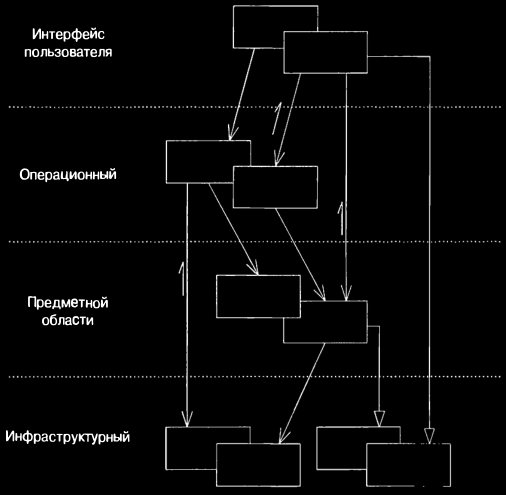
\includegraphics[height=0.8\textheight]{layersBlack.png}
        \end{center}
    \end{frame}

    \begin{frame}
        \frametitle{Изоляция предметной области, соображения}
        \begin{itemize}
            \item Модель предметной области должна быть отделена от остальной программы
            \item Классы модели умеют делать только ``суть''
            \item Сборка всего воедино и общее управление процессом --- на операционный уровень
            \begin{itemize}
                \item Бизнес-регламенты --- на уровне модели предметной области
            \end{itemize}
            \item Все технические вещи --- на инфраструктурный уровень
            \begin{itemize}
                \item Работа с БД
                \item Middleware, сетевые коммуникации
                \item Утилиты
                \item Абстрактные базовые классы
            \end{itemize}
            \item Observer или вариации MVC для связей ``снизу вверх''
        \end{itemize}
    \end{frame}

    \begin{frame}
        \frametitle{Антипаттерн ``Умный GUI''}
        \begin{itemize}
            \item А давайте всю бизнес-логику писать прямо в обработчиках на форме
            \item Код GUI напрямую работает с БД
            \item Делает невозможным проектирование по модели
            \item Не всегда плохо
            \begin{itemize}
                \item Применимы средства быстрой разработки приложений
                \item Прирост производительности на начальных этапах
                \item Легко приделывать новые фичи и переписывать старые
            \end{itemize}
            \item Не всегда хорошо
            \begin{itemize}
                \item Очень сложно переиспользование
                \item Сложно реализовать сложное поведение (зато легко простое)
                \item Сложно интегрироваться
            \end{itemize}
        \end{itemize}
    \end{frame}

    \begin{frame}
        \frametitle{Основные структурные элементы модели}
        \begin{itemize}
            \item \textbf{Сущность (Entity)} --- объект, обладающий собственной идентичностью
            \begin{itemize}
                \item Нужна операция идентификации
                \item Нужен способ поддержания идентичности
            \end{itemize}
            \item \textbf{Объект-значение (Value object)} --- объект, полностью определяемый своими атрибутами
            \begin{itemize}
                \item ``Лучше'', чем сущность
                \item Как правило, немутабельны
                \item Могут быть разделяемыми
            \end{itemize}
            \item \textbf{Служба (Service)} --- объект, представляющий операцию
            \begin{itemize}
                \item Как правило, не имеет собственного состояния
                \item Операции нет естественного места в других классах модели
            \end{itemize}
            \item \textbf{Модуль (Module)} --- смысловые части модели
        \end{itemize}
    \end{frame}

    \begin{frame}
        \frametitle{Жизненный цикл объекта}
        \begin{center}
            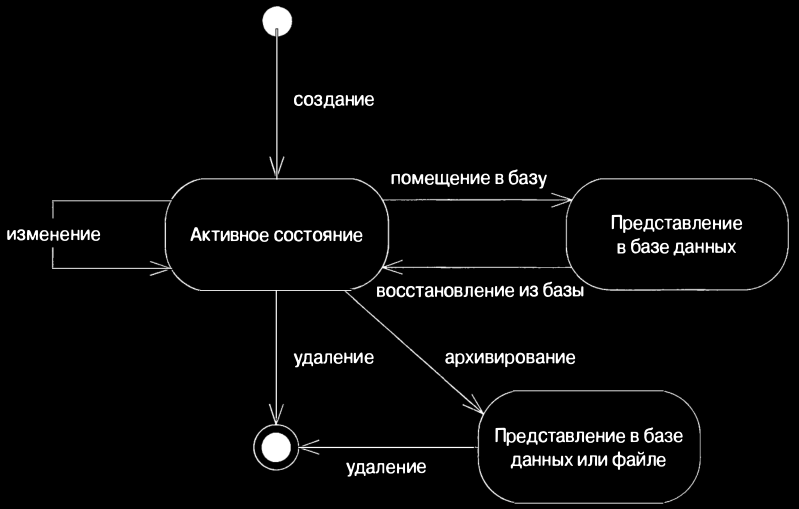
\includegraphics[height=0.7\textheight]{objectLifeCycleBlack.png}
        \end{center}
    \end{frame}

    \begin{frame}
        \frametitle{Агрегаты}
        \begin{itemize}
            \item \textbf{Агрегат} --- изолированный кусок модели, имеющий \textbf{корень} и \textbf{границу}
            \item Корень --- глобально идентичный объект-сущность
            \item Остальные объекты в агрегате идентичны локально
            \item Извне агрегата можно хранить ссылку только на корень
            \begin{itemize}
                \item Отдавать временную ссылку можно
            \end{itemize}
            \item Корень отвечает за поддержание инвариантов всего агрегата
        \end{itemize}
    \end{frame}

    \begin{frame}
        \frametitle{Агрегат, пример}
        \begin{center}
            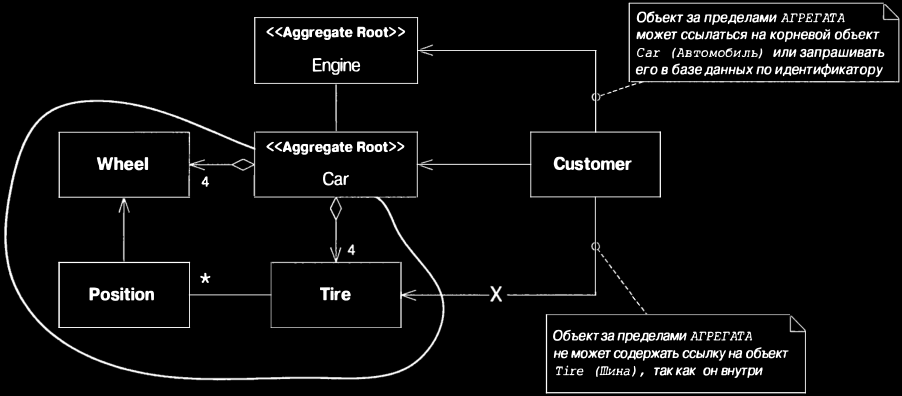
\includegraphics[width=0.9\textwidth]{aggregateBlack.png}
        \end{center}
    \end{frame}

    \begin{frame}
        \frametitle{Фабрика}
        \begin{center}
            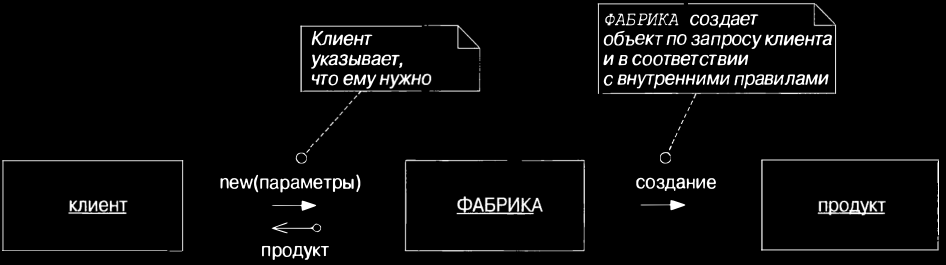
\includegraphics[width=0.7\textwidth]{factoryBlack.png}
        \end{center}
        \textbf{Фабрика} служит для создания объектов или агрегатов
        \begin{itemize}
            \item Скрывает внутреннее устройство конструируемого объекта
            \begin{itemize}
                \item Операция создания ``атомарна'' и обеспечивает инварианты
            \end{itemize}
            \item Изолирует сложную операцию создания
            \item Как правило, не имеет бизнес-смысла, но является частью модели
            \item Реализуется аж несколькими разными паттернами
        \end{itemize}
    \end{frame}

    \begin{frame}
        \frametitle{Пример}
        \framesubtitle{Фабрика, использующаяся для восстановления объекта}
        \begin{center}
            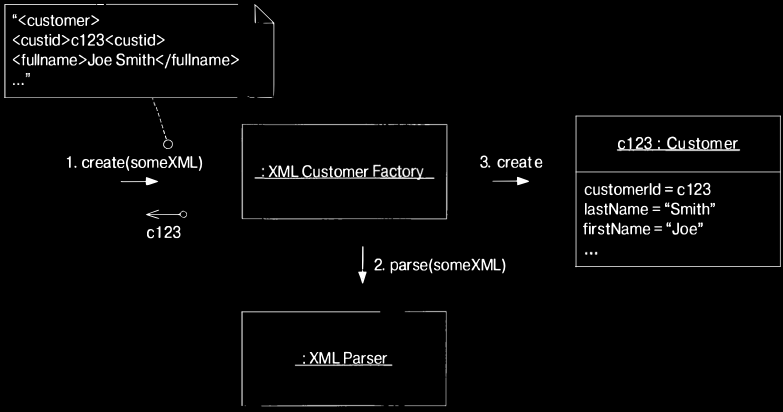
\includegraphics[width=0.8\textwidth]{xmlFactoryBlack.png}
        \end{center}
    \end{frame}

    \begin{frame}
        \frametitle{Хранилище (Repository)}
        \begin{center}
            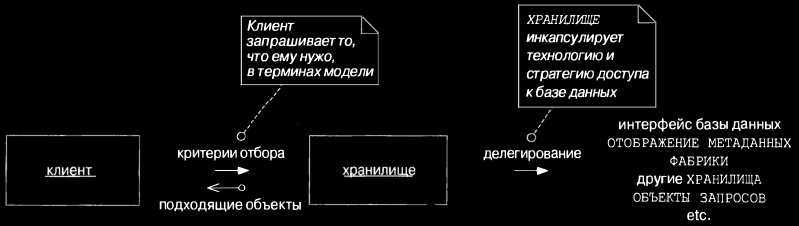
\includegraphics[width=0.8\textwidth]{repositoryBlack.png}
        \end{center}
        \textbf{Репозиторий} хранит объекты и предоставляет к ним доступ
        \begin{itemize}
            \item Может инкапсулировать запросы к БД
            \item Может использовать фабрики
            \item Может обладать развитым интерфейсом запросов
        \end{itemize}
    \end{frame}

    \section{Пример: система грузоперевозок}

    \begin{frame}
        \frametitle{Пример, система грузоперевозок}
        Требования:
        \begin{enumerate}
            \item Отслеживать ключевые манипуляции с грузом клиента
            \item Оформлять заказ заранее
            \item Автоматически высылать клиенту счет-фактуру по достижении грузом некоторого операционного пункта маршрута
        \end{enumerate}

        \begin{itemize}
            \item В работе с Грузом (Cargo) участвует несколько Клиентов (Customers), каждый из которых играет свою роль (Role)
            \item Должна задаваться (bе specified) цель (goal) доставки груза
            \item Цель (goal) доставки груза достигается в результате последовательности Переездов (Carrier Movement), которые удовлeтворяют Заданию (Specification)
        \end{itemize}
    \end{frame}

    \begin{frame}
        \frametitle{Модель}
        \begin{center}
            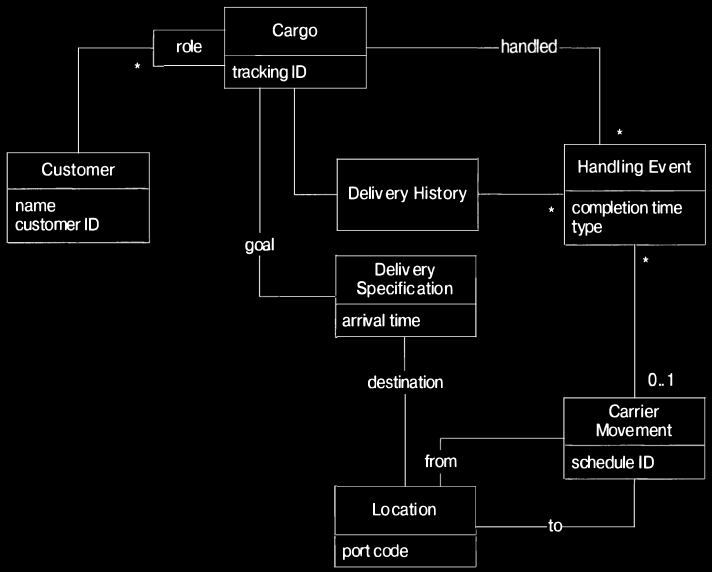
\includegraphics[width=0.7\textwidth]{cargoModelBlack.png}
        \end{center}
    \end{frame}

    \begin{frame}
        \frametitle{Уровень приложения}
        Применим уровневую архитектуру и выделим операции уровня приложения:
        \begin{itemize}
            \item Мaршрутный запрос (Tracking Query) --- манипуляции с конкретным грузом
            \item Служба резервирования (Booking Application) --- позволяет заказать доставку нового груза
            \item Служба регистрации событий (Incident Logging Application) --- регистрирует действия с грузом (связана с маршрутным запросом)
        \end{itemize}
    \end{frame}

    \begin{frame}
        \frametitle{Сущности или значения?}
        \begin{itemize}
            \item \textbf{Клиент (Customer)} --- сущность
            \item \textbf{Груз (Cargo)} --- сущность
            \item \textbf{Манипуляция (Handling Event)} и \textbf{Переезд (Carrier Movement)} --- сущности
            \item \textbf{Местоположение (Location)} --- сущность
            \item \textbf{История доставки (Delivery History)} --- сущность, локально идентична в пределах агрегата ``Груз''
            \item \textbf{Задание на доставку (Delivery Specification)} --- значение
            \item Всё остальное --- значения
        \end{itemize}
    \end{frame}

    \begin{frame}
        \frametitle{Направленность ассоциаций}
        \begin{center}
            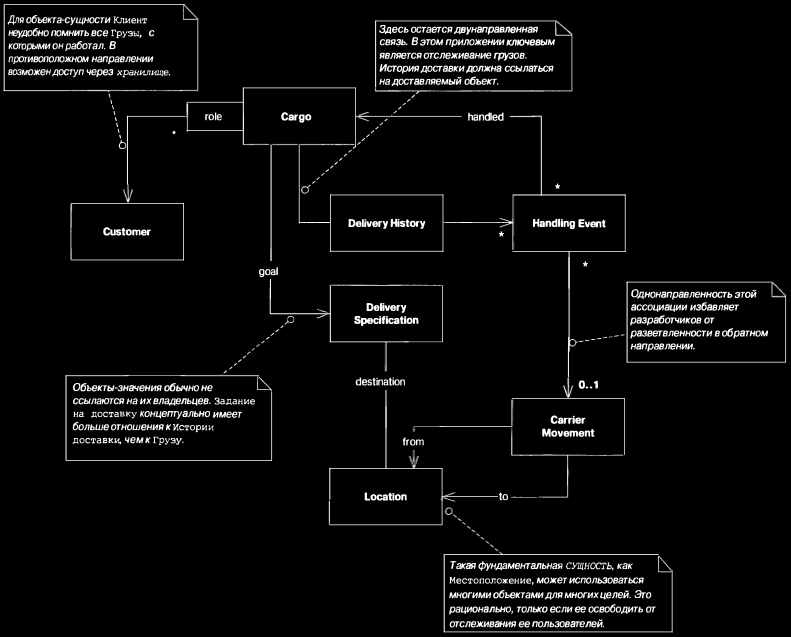
\includegraphics[width=0.8\textwidth]{cargoAssociationsBlack.png}
        \end{center}
    \end{frame}

    \begin{frame}
        \frametitle{Границы агрегатов}
        \begin{center}
            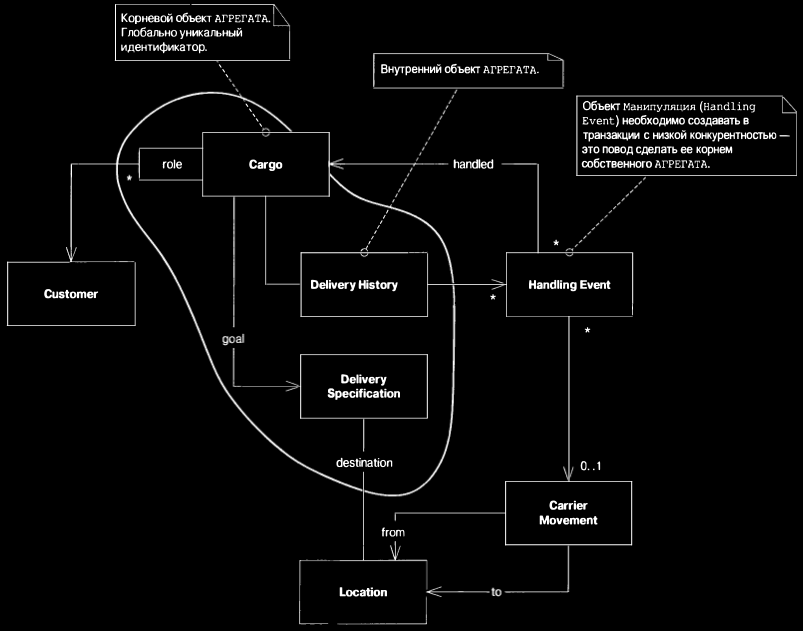
\includegraphics[width=0.82\textwidth]{cargoAggregatesBlack.png}
        \end{center}
    \end{frame}

    \begin{frame}
        \frametitle{Хранилища}
        \begin{center}
            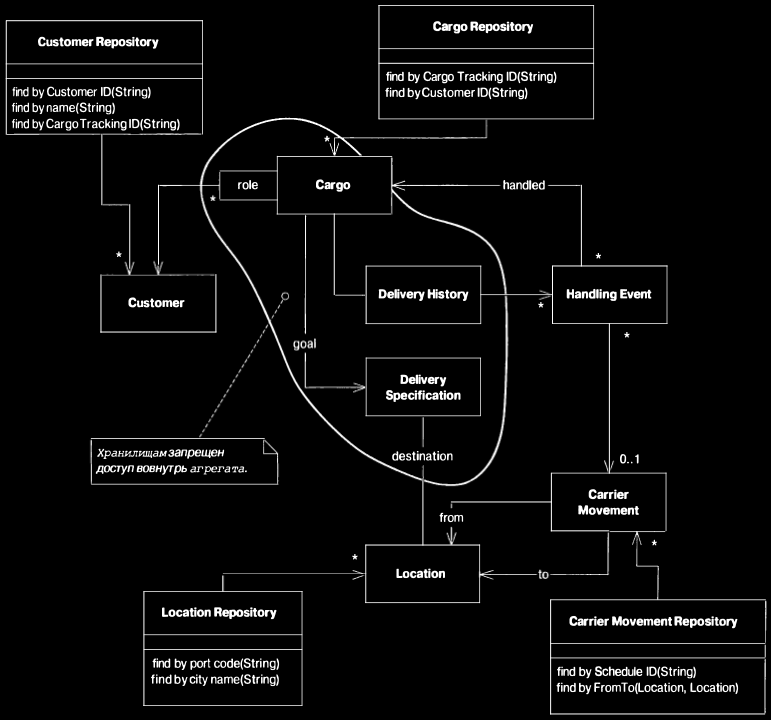
\includegraphics[width=0.75\textwidth]{cargoRepositoriesBlack.png}
        \end{center}
    \end{frame}

    \begin{frame}
        \frametitle{Тестовый сценарий, добавление события}
        \begin{center}
            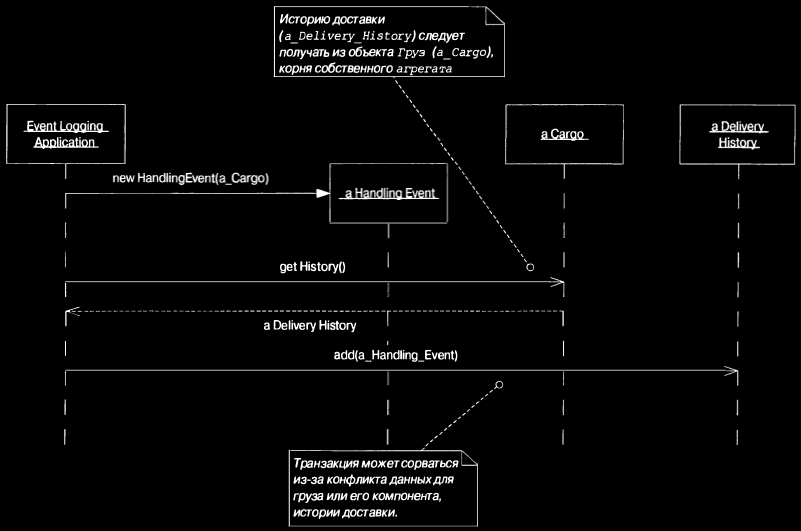
\includegraphics[width=0.9\textwidth]{cargoAddEventBlack.png}
        \end{center}
    \end{frame}

    \begin{frame}
        \frametitle{Рефакторинг, не хранить события явно}
        \begin{center}
            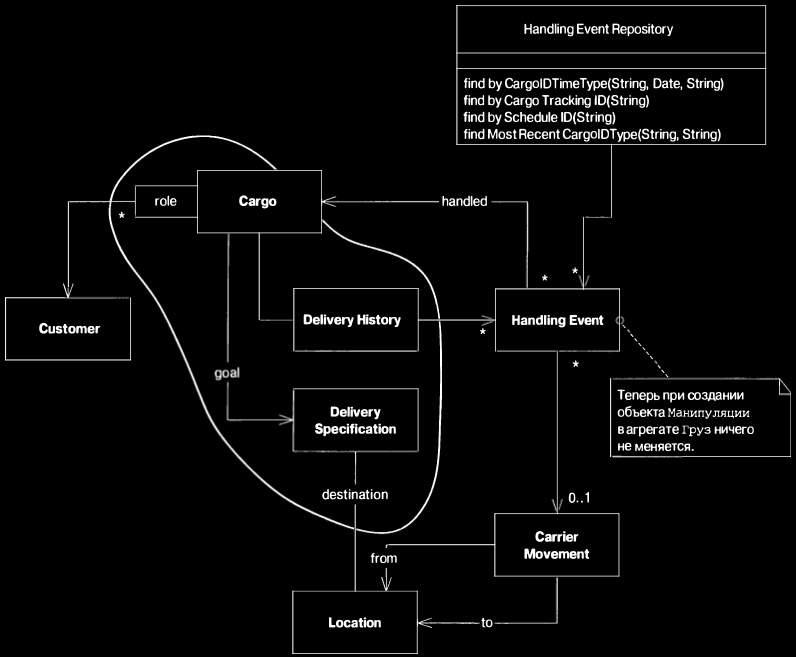
\includegraphics[width=0.85\textwidth]{cargoRefactoredBlack.png}
        \end{center}
    \end{frame}

    \begin{frame}
        \frametitle{Разбиение по модулям, плохо}
        \begin{center}
            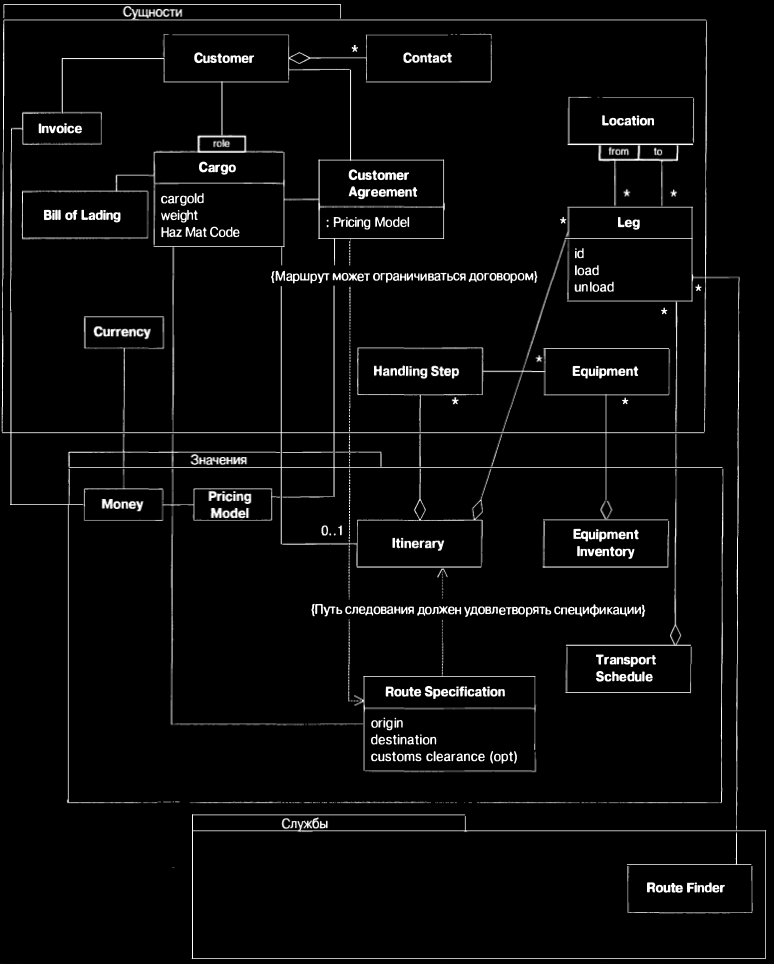
\includegraphics[height=0.8\textheight]{cargoModulesBadBlack.png}
        \end{center}
    \end{frame}

    \begin{frame}
        \frametitle{Разбиение по модулям, хорошо}
        \begin{center}
            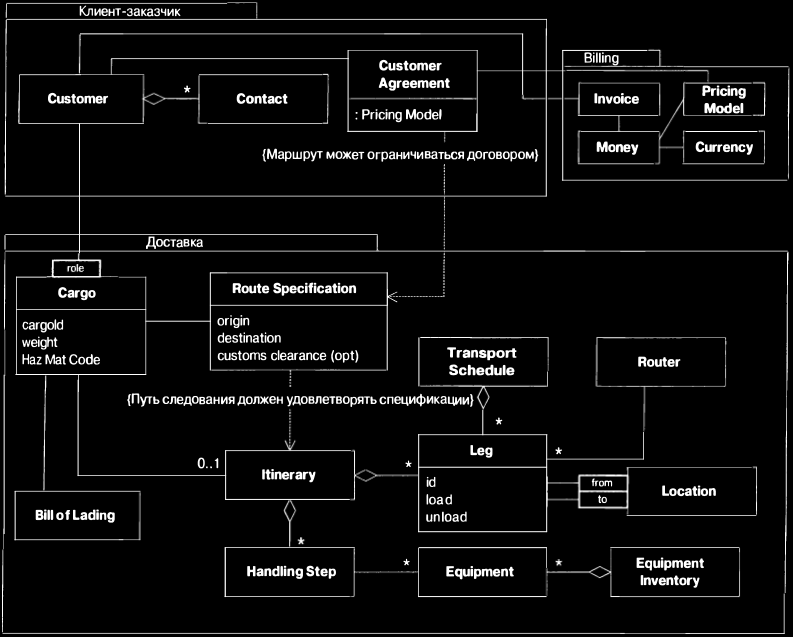
\includegraphics[height=0.8\textheight]{cargoModulesGoodBlack.png}
        \end{center}
    \end{frame}

    \section{Моделирование ограничений}

    \begin{frame}
        \frametitle{Моделирование ограничений}
        \framesubtitle{Простой пример}
        \begin{center}
            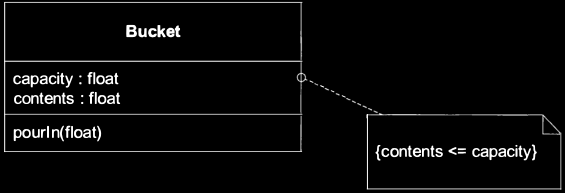
\includegraphics[width=0.6\textwidth]{bucketBlack.png}
        \end{center}
    \end{frame}

    \begin{frame}[fragile]
        \frametitle{Код, до}
        \begin{minted}{java}
class Bucket {
    private float capacity;
    private float contents;

    public void pourIn(float addedVolume) {
        if (contents + addedVolume > capacity) {
            contents = capacity;
        } else {
            contents = contents + addedVolume;
    }
}
        \end{minted}
    \end{frame}

    \begin{frame}[fragile]
        \frametitle{Код, после}
        \begin{minted}{java}
class Bucket {
    private float capacity;
    private float contents;

    public void pourIn(float addedVolume) {
        float volumePresent = contents + addedVolume;
        contents = constrainedToCapacity(volumePresent);
    }

    private float constrainedToCapacity(float volumePlacedIn) {
        if (volumePlacedIn > capacity) return capacity;
        return volumePlacedIn;
    }
} 
        \end{minted}
    \end{frame}

    \begin{frame}
        \frametitle{Паттерн ``Спецификация''}
        \begin{center}
            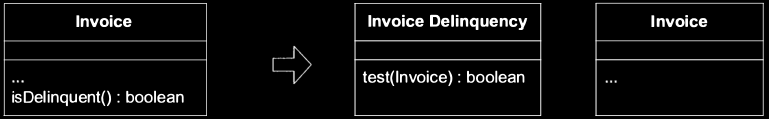
\includegraphics[width=0.8\textwidth]{specificationBlack.png}
        \end{center}
        \textbf{Спецификация} инкапсулирует ограничение в отдельном объекте
        \begin{itemize}
            \item Предикат
            \item Может быть использована для выборки или конструирования объектов
        \end{itemize}
    \end{frame}

    \begin{frame}
        \frametitle{Композитные спецификации}
        \begin{center}
            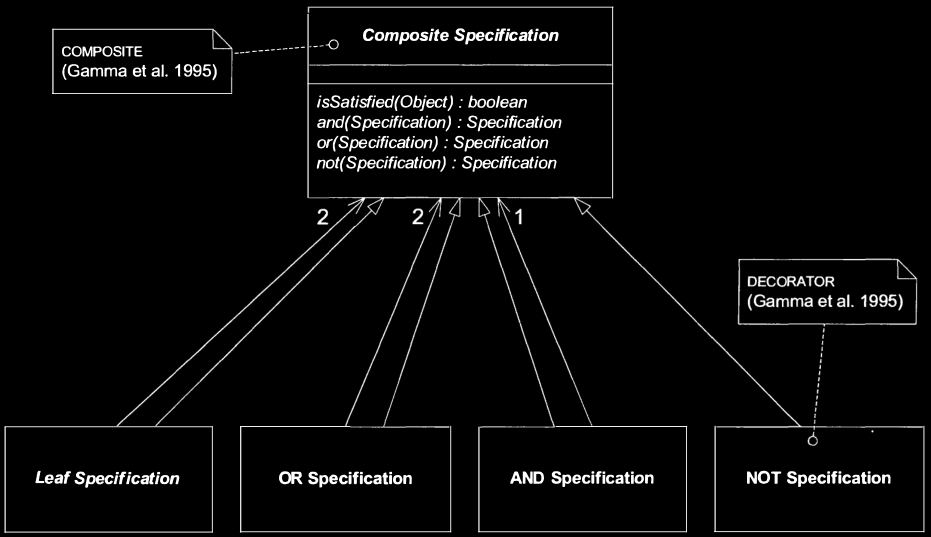
\includegraphics[height=0.7\textheight]{compositeSpecificationsBlack.png}
        \end{center}
    \end{frame}

    \begin{frame}
        \frametitle{Пример: склад химикатов}
        \begin{center}
            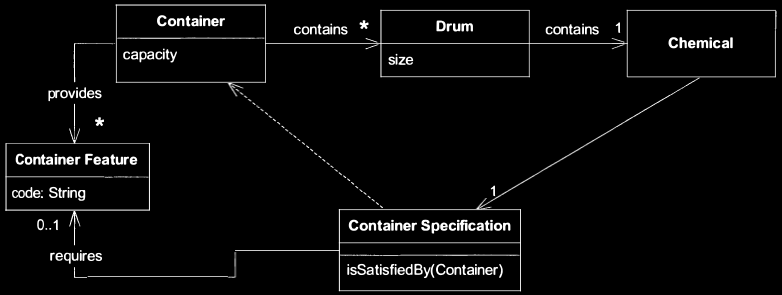
\includegraphics[width=0.9\textwidth]{chemicalsStructureBlack.png}
        \end{center}
    \end{frame}

    \begin{frame}[fragile]
        \frametitle{Код, спецификация}
        \begin{minted}{java}
public class ContainerSpecification {
    private ContainerFeature requiredFeature;

    public ContainerSpecification(ContainerFeature required) {
        requiredFeature = required;
    }

    boolean isSatisfiedBy(Container aContainer) {
        return aContainer.getFeatures().contains(requiredFeature);
    }
}
        \end{minted}
    \end{frame}

    \begin{frame}[fragile]
        \frametitle{Код, контейнер}
        \begin{minted}{java}
boolean isSafelyPacked() {
    Iterator it = contents.iterator();
    while (it.hasNext()) {
        Drum drum = (Drum) it.next() ;
        if (!drum.containerSpecification().isSatisfiedBy(this))
            return false ;
    }
    return true;
}
        \end{minted}
    \end{frame}

\end{document}
